\clearpage
\section{Automatyzacja i centralizacja wersjonowania projektu (JC)}
\label{ch:versioning}

Niniejszy rozdział traktuje o wersjonowaniu w projekcie ggss. Sposobie w jaki były wersjonowane aplikacje przed wprowadzeniem najnowszych zmian, wymaganiami jakie zostały postawione co do systemu wersjonowania oraz sposobie implementacji wymaganego systemu wersjonowania.

\subsection{Wprowadzenie do problematyki}

Wersjonowanie oprogramowania jest to proces, którego celem jest przypisanie aplikacji utworzonej danego dnia unikatowego identyfikatora, dzięki czemu w dowolnej chwili jesteśmy w stanie wrócić do aplikacji, która już wcześniej znajdowała się w środowisku produkcyjnym i została dogłębnie przetestowana. Jest to szczególnie przydatne w momencie, gdy z jakiegoś powodu do środowiska produkcyjnego trafi zepsuta wersja aplikacji. Ponadto wersjonowanie aplikacji pozwala na śledzenie zmian oraz wprowadzanych usprawnień w aktualizacji. Użytkownicy są w stanie, sprawdzjąc dokumentację wprowadzonych zmian, określić, czy wersja aplikacji którą używają posiada wszystkie wymagane przez nich funkcjonalności. Ponadto znajdywanie głownej przyczyny późno wykrytego błędu staje się znacznie prostrze. Jest możliwe porównanie różnych wersji aplikacji, dzięki czemu możliwe jest określnie w jakim przedziale czasowym pojawił się wyżej wymieniony błąd.

W projekcie ggss wersjonowaniu poddawany był jedynie pakiet RPM z sterownikami oraz zależnościami zewnętrznymi. Wersja składała się z czterech komponentów, czyli \lstinline{<MAJOR>.<MINOR>.<PATCH>-<RELEASE>}. Komponent wersji, który był zmieniany przy wprowadzaniu zmian był wybierany uznaniowo. Dodatkowo wersjonowanie do tej pory było rozwiązane jako ręcznie wpisana wartość w plikach CMake służących do budowania projektu. Każda z części projektu ggss, która wymagała wersjonowania była wersjonowana osobno.

\subsection{Motywacja do wprowadzenia zmian}

Pierwszym czynnikiem, z powodu którego zdecydowano się na wprowadzenie zmian w systemie wersjonowania była jego nieporęczność. Każda zmiana i wydanie nowej wersji aplikacji wymagały od dewelopera, aby pamiętał, że należy jeszcze dodatkowo zmienić wersję w plikach CMake. Był to kolejny krok który programista musiał wykonać w celu przeprowadzenia poprawnego procesu rozwoju oprogramowania, a co za tym idzie potencjalnie kolejne miejsce na pomyłkę. Dodatkowo nieodpowiednia zmiana wersji, na przykład przez pomyłkę, na niższą powodowała problemy z procesem instalacji nowej wersji oprogramowania w środowisku docelowym. Ze względu na to, że systemy działające przy detektorze mają bardzo duże restrykcje proces instalacji nowych wersji aplikacji jest monitorowany przez administratorów systemowych. Pomyłki w zmianie wersji oprogramowania uniemożliwiały ich zainstalowanie ze względu na błędy w działaniu menadżera pakietów oraz sprzeciw administratorów dla instalacji niepoprawnie wersjonowanych aplikacji.

Kolejnym czynnikiem który spowodował wprowadzenie zmian w systemie wersjonowania był wymóg postawiony autorom, aby wszystkie aplikacje ggss publikowane w danym momencie miały dokładnie tą samą wersję, to jest: aby zarówno komponent A miał wersję X, jak i komponent B miał wersję X. Dzięki zastosowaniu takiego podejścia możliwe jest bardzo szybkie zidentyfikowanie kombinacji komponentów systemu ggss, które są ze sobą kompatybilne.

Ze względu na te czynniki postanowiono przygotować zautomatyzowany, scentralizowany system wersjonowania oparty o dostępną infrastrukturę, czyli: skrypty budujące w języku Python, pliki CMake, portal Gitlab i automatyzację w oparciu o Gitlab CI/CD.

\subsection{Zmiany w skryptach budujących projekt}

W celu zapewnienia automatycznego, scentralizowanego wersjonowania należało wykonać zmiany w kilku warstwach projektu ggss. W pierwszej kolejności zmodyfikowano głowny skrypt do budowania (\lstinline{build.py}) w repozytorium ggss-all. Została dodana do niego obsługa argumentu wejściowego \lstinline{--version} tak, aby można było definiować wersję zarówno ręcznie w trakcie uruchamiania wyżej wymienionego skryptu, jak i poprzez automatyzację zdefiniowaną w ramach Gitlab CI/CD. W przypadku braku podania wersji, którą mają zostać oznaczone budowane pliki postanowiono ustawiać ją tak, aby było wiadomo, że wyprodukowane pliki stanowią wersję deweloperską, a nie produkcyjną. W takim przypadku wersja przygotowywana przez skrypt wygląda następująco: \lstinline{dev-YYYY-MM-DD_HH-MM-SS}. Pozwala to na identyfikację, że pliki zostały zbudowane poza oficjalnym systemem automatyzującym cały proces, oraz dokładną datę i godzinę kiedy skrypt budujący został uruchomiony. Oprócz rozszerzenia argumentów wejściowych dostosowania wymagał również sposób obsługi plików CMake w wyżej wymienionym skrypcie. Wersja przekazywania jest za pomocą parametru \lstinline{VERSION} do wszystkich plików CMake obsługiwanych przez skrypt.

\subsection{Zmiany w plikach CMake}

W przypadku plików CMake zasotosowano podobne podejście, jak w przypadku pliku \lstinline{build.py}. Dodano argument wejściowy w postaci parametru \lstinline{VERSION}. Pozwala to na odebranie wartości wersji od skryptów zewnętrznych, jak i ręcznie wpisanej przez użytkownika korzystającego z plików CMake. W przypadku nieustawienia wartości wyżej wymienionego parametru ustawiana jest wartość domyślna w postaci \lstinline{no-version}. Listing \ref{lst:cmake_version_arg} przedstawia przykładowe zastosowanie tego systemu w przypadku repozytorium ggss-driver.

\begin{lstlisting}[language=CMake,caption={Zastosowanie parametru VERSION w repozytorium ggss-driver},label={lst:cmake_version_arg},frame=single]
if(NOT VERSION)
    set(VERSION "no-version")
endif()

message(STATUS "ggss-driver version: ${VERSION}")

#parameter initialization
set (CPACK_PACKAGE_NAME "ggss-driver-cc7")
set (CPACK_PACKAGE_VERSION ${VERSION})
\end{lstlisting}


\subsection{Zastosowanie semantic-versioning oraz zmiany w automatyzacji}
%dwa nowe stage od semantic versioning, analiza commitów, tworzenie nowych release

Do tej pory w projekcie ggss wersja była zmieniania według uznania dewelopera, który wprowadzał tą informację w plikach CMake odpowiedzialnych za budowanie danego komponentu aplikacji. W celu ustandaryzowania tego procesu zdecydowano się na stosowanie zasad \emph{semantic-versioning}. Według tychże zasad wersja składa się z trzech komponentów, tj.:
\begin{itemize}
    \item MAJOR - komponent ten jest zmieniany, gdy wprowadzamy zmiany w API aplikacji, które nie są kompatybilne z wcześniejszymi wydaniami, na przykład: dodatkowy, wymagany argument bez wartości domyślnej
    \item MINOR - komponent ten jest zmieniany, gdy wprowadzamy zmiany w aplikacji, które są kompatybilne z wcześniejszymi wydaniami, na przykład: dodanie nowej całkowicie funkcjonalności, które nie wpływa na pozostałe dotąd oferowane możliwości
    \item PATCH - komponent ten jest zmieniamy, gdy wprowadzamy poprawki, które są kompatybilne z wcześniejszymi wydaniami, na przykład: poprawa błędu wykrytego w aplikacji, zwiększenie stabilności
\end{itemize}
Zmieniając komponent o większym znaczeniu, należy wyzerować pozostałe komponenty wersji, czyli zmieniając wersję MAJOR należy wyzerować zarówno MINOR, jak i PATCH.

Oprócz zastosowania wyżej wymienionych zasad postanowiono udoskonalić cały system wersjonowania o automatyzację za pomocą pipeline GitLab CI/CD. W tym celu wykorzystano projekt \emph{semantic-release}. Jest to projekt oparty o język JavaScript uruchamiany w środowisku NodeJS. Projekt ten pobiera informacje zawarte w rewizjach oraz na portali Gitlab dotyczące repozytorium w ramach którego został uruchomiony. Następnie pozyskane dane analizuje w celu określenia, czy powinna zostać uruchomiona automatyzacja odpowiedzialna za utworzenia nowego wydania (ang. release) na platformie Gitlab wraz z zwiększeniem wersji wg zasad semantic-versioning.

Ze względu na to, że informacje na temat wersji potrzebne są również w części automatyzacji odpowiedzialnej za budowanie aplikacji podzielono wykorzystano projektu semantic-release na dwa kroki. W pierwszej kolejności uruchamiana jest analiza wiadomości zawartych w ramach rewizji tak, aby określić, czy wersja powinna zostać zmieniona oraz który komponent wersji powinien zostać zmieniony. Następnie informacja o wersji przekazywana jest do kroku odpowiedzialnego za budowanie wszystkich aplikacji projektu ggss. W ostatnim kroku gotowe do użycia aplikacje są przekazywane drugiego kroku wykonywanego w ramach logiki semtantic-release, czyli utworzenie nowego wydania. Rysunek \ref{fig:semantic_pipeline} przedstawia kroki podejmowane w ramach procesu automatyzacji. W ramach kroku ``Prepare`` przygotowywana jest informacja o wersji, w ramach kroku ``Build`` budowane są wszystkie aplikacjie biorąc pod uwagę wcześniej przygotowaną wersją, a w ramach kroku ``Releasse`` tworzona jest nowe wydanie.

\begin{figure}[H]
    \centering
    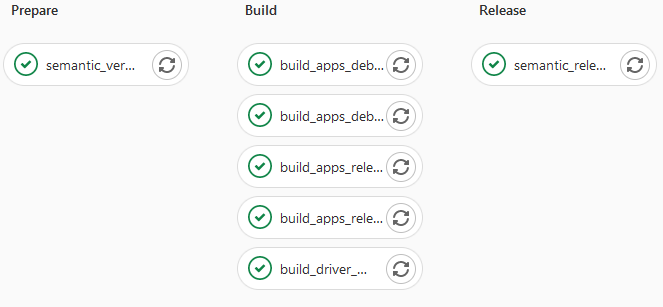
\includegraphics[width=0.9\textwidth]{semantic_release_pipeline}
    \caption{Kroki procesu automatyzacji z wykorzystaniem semantic-versioning.}
    \label{fig:semantic_pipeline}
\end{figure}

Zasady analizy wiadomości w ramach rewizji przez semantic-release również zostały ustandaryzowane, a określone są przez konwencję \emph{ESLint}. W przypadku, gdy powinno zostać utworzone nowe wydanie należy wraz z nową rewizją przygotować wiadomośc w następującym formacie: \lstinline{tag: opis}, gdzie tag to jedna z następujących wartości:
\begin{itemize}
    \item Fix - naprawa błędu
    \item Update - usprawnienie kompatybilne wstecz
    \item New - nowa funkcjonalność
    \item Breaking - zmiany niekompatybilne wstecz
    \item Docs - zmiany w dokumentacji
    \item Build - zmiany w procesie budowania
    \item Upgrade - zmiany w zależnościach
    \item Chore - zmiany, które w żaden sposób nie wpływają na użytkowanie, np.: zmiany w testach
\end{itemize}
Opisem może być dowolna wiadomośc krótko podsumowująca dokonane zmiany. Na podstawie analizowanych tagów semantic-release stosując zasady semantic-versioning automatycznie ustala odpowiednią informację o wersji. Przykładowe działania projektu semantic-release zostało przedstawione na listingu \ref{lst:analyze}.


\begin{lstlisting}[language=cmd, caption={Analiza wiadomości zawartych w rewizjach z wykorzystaniem semantic-release.}, label={lst:analyze}]
[@semantic-release/commit-analyzer] > Analyzing commit: Breaking: This is for presentation reasons
[@semantic-release/commit-analyzer] > The release type for the commit is major
[@semantic-release/commit-analyzer] > Analysis of 29 commits complete: major release
[semantic-release] > Completed step "analyzeCommits" of plugin "@semantic-release/commit-analyzer"
[semantic-release] > The next release version is 1.0.0
\end{lstlisting}

\subsection{Podsumowanie}

Dzięki zastosowaniu wszystkich kroków przedstawionych w ramach zagadnienia wersjonowania osiągnięto w projekcie ggss scentralizowany, zautomatyzowany system wersjonowania wydań aplikacji. Wszystkie kroki potrzebne do utrzymania odpowiedniej wersji odbywają się w ramach automatyzacji opartej o Gitlab CI/CD oraz projekt semantic-release. Deweloper musi jedynie wprowadzać odpowiednie oznaczenia w wiadomościach związanych z kolejnymi rewizjami, a utworzony system automatycznie zajmie się ewaluacją wszystkich trzech komponentów kolejnej wersji, zbuduje wszystkie aplikacje przekazując wcześniej uzyskane dane oraz udostępni gotowe do działania aplikacjie w ramach nowego wydania dostępnego na portalu Gitlab.

%https://semver.org/
%https://github.com/semantic-release/semantic-release
%https://github.com/conventional-changelog/conventional-changelog/tree/master/packages/conventional-changelog-eslint